\section{Internal coordinates of \texorpdfstring{\pa}{CH3CNH+} }


\subsection{fc-CCSD(T)/ANO0}
\begin{verbatim}

H
C 1 r1
C 2 r2 1 a1
X 3 rd 2 a90 1 d0
N 3 r3 4 a90 2 d180
X 5 rd 3 a90 4 d0
H 5 r4 6 a90 3 d180
H 2 r1 3 a1 1 d120
H 2 r1 3 a1 8 d120

r1   =        1.097234034575213
r2   =        1.461586511773973
a1   =      108.354029317585457
rd   =        1.000000409314806
a90  =       89.999999999999972
d0   =        0.000000000000000
r3   =        1.153699023716097
d180 =      180.000000000000000
r4   =        1.013272030286403
d120 =      120.000000000000114

\end{verbatim}
    
\subsection{fc-CCSD(T)/ANO1}

\begin{verbatim}

H
C 1 r1
C 2 r2 1 a1
X 3 rd 2 a90 1 d0
N 3 r3 4 a90 2 d180
X 5 rd 3 a90 4 d0
H 5 r4 6 a90 3 d180
H 2 r1 3 a1 1 d120
H 2 r1 3 a1 8 d120

r1   =        1.091588568955683
r2   =        1.450334012198720
a1   =      108.507798899076860
rd   =        1.000000613972271
a90  =       89.999999999999986
d0   =        0.000000000000000
r3   =        1.145583771122200
d180 =      180.000000000000000
r4   =        1.008294043229717
d120 =      119.999999999999972

\end{verbatim}

\subsection{fc-CCSD(T)/ANO2}
\begin{verbatim}

H
C 1 r1
C 2 r2 1 a1
X 3 rd 2 a90 1 d0
N 3 r3 4 a90 2 d180
X 5 rd 3 a90 4 d0
H 5 r4 6 a90 3 d180
H 2 r1 3 a1 1 d120
H 2 r1 3 a1 8 d120

r1   =        1.090663342780039
r2   =        1.448609574844010
a1   =      108.480759568085148
rd   =        1.000001227944922
a90  =       90.000000000000028
d0   =        0.000000000000000
r3   =        1.142864353443497
d180 =      180.000000000000000
r4   =        1.008334309784723
d120 =      120.000000000000327

\end{verbatim}

\subsection{fc-CCSD(T)/cc-pVDZ}
\begin{verbatim}

H
C 1 r1
C 2 r2 1 a1
X 3 rd 2 a90 1 d0
N 3 r3 4 a90 2 d180
X 5 rd 3 a90 4 d0
H 5 r4 6 a90 3 d180
H 2 r1 3 a1 1 d120
H 2 r1 3 a1 8 d120

r1   =        1.104421287381395
r2   =        1.467855029147642
a1   =      108.258731223153745
rd   =        1.000000409314806
a90  =       89.999999999999957
d0   =        0.000000000000000
r3   =        1.160263599078930
d180 =      180.000000000000000
r4   =        1.020376191984162
d120 =      120.000000000000171

\end{verbatim}

\subsection{fc-CCSD(T)/cc-pVTZ}
\begin{verbatim}

H
C 1 r1
C 2 r2 1 a1
X 3 rd 2 a90 1 d0
N 3 r3 4 a90 2 d180
X 5 rd 3 a90 4 d0
H 5 r4 6 a90 3 d180
H 2 r1 3 a1 1 d120
H 2 r1 3 a1 8 d120

r1   =        1.091362895166567
r2   =        1.453075807535473
a1   =      108.438787022956490
rd   =        1.000000204657382
a90  =       89.999999999999986
d0   =        0.000000000000000
r3   =        1.146078556823367
d180 =      180.000000000000000
r4   =        1.009021121407080
d120 =      120.000000000000099

\end{verbatim}

\subsection{ae-CCSD(T)/cc-pwCV5Z}
\begin{verbatim}

H
N 1 r1*
X 2 rd 1 a90
C 2 r2* 3 a90 1 d180
X 4 rd 2 a90 3 d0
C 4 r3* 5 a90 2 d180
H 6 r4* 4 a1* 5 d0
H 6 r4* 4 a1* 7 d120
H 6 r4* 4 a1* 8 d120

r1   =        1.0073314907
rd   =        1.0
a90  =       90.0
r2   =        1.1399556988
d180 =      180.000000000000000
d0   =        0.000000000000000
r3   =        1.4440897526
r4   =        1.0887809197
a1   =      108.5586585536
d120 =      120.0

\end{verbatim}

\section{Internal coordinates of \texorpdfstring{\pan}{CH3CNH+-Ne} -Ne }

\subsection{fc-CCSD(T)/ANO0}

\begin{verbatim}

H
C 1 r1
C 2 r2 1 a1
X 3 rd 2 a90 1 d0
N 3 r3 4 a90 2 d180
X 5 rd 3 a90 4 d0
H 5 r4 6 a90 3 d180
H 2 r1 3 a1 1 d120
H 2 r1 3 a1 8 d120
X 7 rd 5 a90 6 d0
NE 7 r5 10 a90 5 d180

r1   =        1.097234259132258
r2   =        1.461586810898442
a1   =      108.354029317585457
rd   =        1.000000613972271
a90  =       89.999999999999972
d0   =        0.000000000000000
r3   =        1.153699259829119
d180 =      180.000000000000000
r4   =        1.013272237660004
d120 =      119.999999999999758
r5   =        2.117272059249112

\end{verbatim}

\subsection{fc-CCSD(T)/cc-pVDZ}
\begin{verbatim}

H
C 1 r1
C 2 r2 1 a1
X 3 rd 2 a90 1 d0
N 3 r3 4 a90 2 d180
X 5 rd 3 a90 4 d0
H 5 r4 6 a90 3 d180
H 2 r1 3 a1 1 d120
H 2 r1 3 a1 8 d120
X 7 rd 5 a90 6 d0
NE 7 r5 10 a90 5 d180

r1   =        1.097234483689349
r2   =        1.461587110022973
a1   =      108.354029317585457
rd   =        1.000000818629779
a90  =       89.999999999999972
d0   =        0.000000000000000
r3   =        1.153699495942189
d180 =      180.000000000000000
r4   =        1.013272445033648
d120 =      119.999999999999758
r5   =        1.990534530346215
\end{verbatim}
\newpage

\newgeometry{left=2.5cm}
% \section{Computed vibrational frequencies}

\begin{landscape}
\begin{center}
\begin{table}[h]
\caption{Computed fc-CCSD(T) vibrational frequencies (in \wn) using ANO basis sets for \pa. }\label{tab:CH3CNH+:tab1}

    \begin{tabular}{llllllllll} \hline\hline\\
            mode        & sym      & exp.$^a$ & \multicolumn{3}{c}{harmonic$^b$}  & \multicolumn{3}{c}{anharmonic (VPT2)$^b$} \\
                        & C$_{3v}$ &      & ANO0        & ANO1       & ANO2       & ANO0        & ANO1      & ANO2 &          \\\hline\\
            $\nu_{10}$  & E	       & 385  & 374 (-11)	& 381  (-4)  & 382  (-3)  & 376  (-9)   & 384 (-1)  & 384  (-1)       \\
            $\nu_9$     & E	       & 596  & 581 (-15)	& 580  (-16) & 585  (-11) & 570  (-26)  & 579 (-17) & 577  (-19)      \\
            $\nu_5$     & A$_1$	   & 898  & 889 (-9)	& 897  (-1)  & 900  (2)   & 878  (-20)  & 887 (-11) & 890  (-8)       \\
            $\nu_8$     & E	       & 1026 & 1051 (25)	& 1048 (22)  & 1050 (24)  & 1025 (-1)   & 1023(-3)  & 1024 (-2)       \\
            $\nu_4$     & A$_1$	   & 1364 & 1395 (31)	& 1393 (29)  & 1398 (34)  & 1358 (-6)   & 1358(-6)  & 1361 (-3)       \\
            $\nu_7$     & E	       & 1421 & 1444 (23)	& 1442 (21)  & 1447 (26)  & 1422 (1)    & 1428(7)   & 1429 (8)        \\
            $\nu_3$     & A$_1$	   & 2307 & 2336 (29)	& 2345 (38)  & 2350 (43)  & 2290 (-17)  & 2300(-7)  & 2305 (-2)       \\
            $\nu_2$     & A$_1$	   & 2924 & 3060 (136)	& 3049 (125) & 3051 (127) & 2934 (10)   & 2927(3)   & 2930 (6)        \\
            $\nu_6$     & E	       & 2996 & 3174 (178)	& 3149 (153) & 3152 (156) & 3019 (23)   & 2999(3)   & 3002 (6)        \\
            $\nu_1$     & A$_1$	   & nc   & 3688 (-)	& 3699 (-)	 & 3687 (-)   & 3528 (-)    & 3534(-)   & 3525 (-)        \\
        \\
        \hline\hline\\
    \end{tabular}
    
    $^a$ This work, Ne-IRPD experiment.\\
    $^b$ Shift from Ne-IRPD experiment is given in parenthesis.
\end{table}
\end{center}
\end{landscape}
\restoregeometry

\begin{table}[h]
\caption{Computed harmonic CCSD(T) vibrational frequencies (in \wn) using Dunning's basis sets for \pa. }\label{tab:CH3CNH+:tab2}
\begin{center}
    \begin{tabular}{llllll} \hline\hline\\
       mode         & sym.  & exp.$^a$  & cc-pVDZ$^b$ & cc-pVTZ$^b$ \\\hline\\
       $\nu_{10}$   & E	    & 385       & 362  (-23)	  & 380  (-5)    \\
       $\nu_9$      & E	    & 596       & 564  (-32)	  & 586  (-10)   \\
       $\nu_5$      & A$_1$	& 898       & 893  (-5)	  & 895  (-3)    \\
       $\nu_8$\     & E	    & 1026      & 1042 (15)  & 1052 (25)  \\
       $\nu_4$      & A$_1$	& 1364      & 1381 (16)  & 1398 (34)  \\
       $\nu_7$      & E	    & 1421      & 1433 (12)  & 1450 (29)  \\
       $\nu_3$      & A$_1$	& 2307      & 2331 (24)  & 2343 (36)  \\
       $\nu_2$      & A$_1$	& 2924      & 3066 (142) & 3052 (128) \\
       $\nu_6$      & E	    & 2996      & 3181 (185) & 3151 (154) \\
       $\nu_1$      & A$_1$	& nc        & 3663 (-)	  & 3684 (-)    \\
        \\
        \hline\hline\\
    \end{tabular}
    
    $^a$ This work, Ne-IRPD experiment.\\
    $^b$ Shift from Ne-IRPD experiment is given in parenthesis.
\end{center}

\end{table}

\begin{table}
\footnotesize
\caption{Computed harmonic CCSD(T) vibrational frequencies (in \wn) comparing both \pa (bare ion) and \pan-Ne (complex) using ANO0 and cc-pVDZ basis sets. }\label{tab:CH3CNH+:tab3}

\begin{center}
    \begin{tabular}{lllllll} \hline\hline\\
    
        mode                    & sym.      & exp.$^a$ & \multicolumn{2}{c}{ANO0$^b$} & \multicolumn{2}{c}{cc-pVDZ$^b$}\\
                                & C$_{3v}$  &      & \pa          & \pan-Ne     & \pa         & \pan-Ne \\ \hline\\
        $\nu_{\mbox{Ne-bend}}$  & E	        &      &              & 32 & 	                 & 26           \\
        $\nu_{\mbox{Ne-str.}}$  & A$_1$	    &      &              & 68 & 	                 & 102          \\
        $\nu_{10}$              & E	        & 385  &  374  (-11)  & 375  (-10) & 362  (-23)	 & 322  (-63)   \\
        $\nu_9$                 & E	        & 596  &  581  (-15)  & 599  (3)   & 564  (-32)	 & 551  (-45)   \\
        $\nu_5$                 & A$_1$	    & 898  &  889  (-9)   & 890  (-8)  & 893  (-5)	 & 913  (15)    \\
        $\nu_8$                 & E	        & 1026 &  1051 (25)   & 1052 (26)  & 1042 (15)	 & 1024 (-2)    \\
        $\nu_4$                 & A$_1$	    & 1364 &  1395 (31)   & 1395 (31)  & 1381 (16)	 & 1370 (6)     \\
        $\nu_7$                 & E	        & 1421 &  1444 (23)   & 1445 (24)  & 1433 (12)	 & 1425 (4)     \\
        $\nu_3$                 & A$_1$	    & 2307 &  2336 (29)   & 2336 (29)  & 2331 (24)	 & 2380 (73)    \\
        $\nu_2$                 & A$_1$	    & 2924 &  3060 (136)  & 3060 (136) & 3066 (142) & 3129 (205)   \\
        $\nu_6$                 & E	        & 2996 &  3174 (178)  & 3173 (177) & 3181 (185) & 3247 (251)   \\
        $\nu_1$                 & A$_1$	    & nc   &  3688 (-)    & 3679 (-)   & 3663 (-)	 & 3730 (-)	    \\

        \\\hline\hline\\
    \end{tabular}\\
    $^a$ This work, Ne-IRPD experiment.\\
    $^b$ Shift from Ne-IRPD experiment is given in parenthesis.
    
\end{center}
\end{table}

\begin{figure}
	\centering
		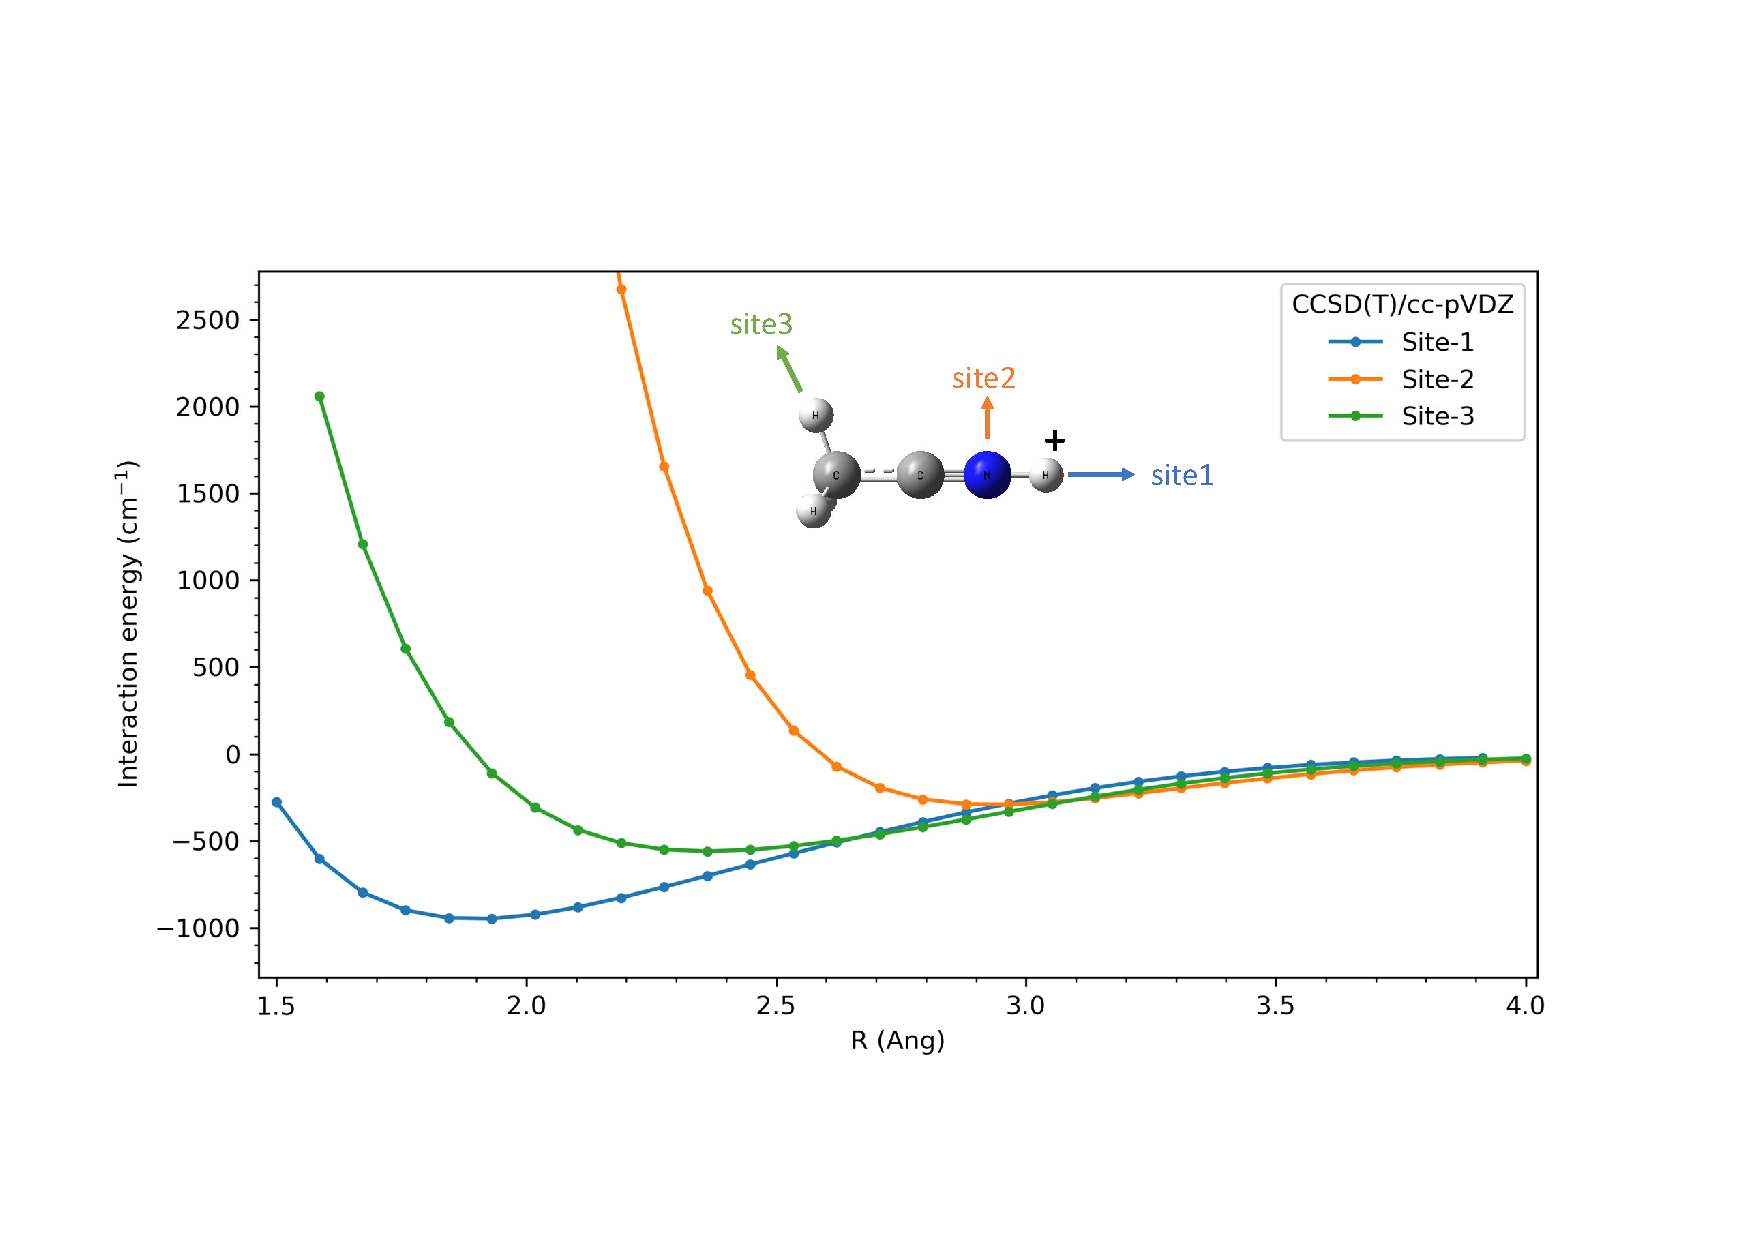
\includegraphics[width=1\textwidth]{chapters/CH3CNH+/figures/iso_comparison_with_Ne.pdf}
		\caption{Computed potential energy surface as a function of Ne distance R for \pan-Ne from various sites neon atom placed.}\label{fig:CH3CNH+:fig1}
	% \label{FIG:bsse}
\end{figure}

\begin{figure}

	\centering
		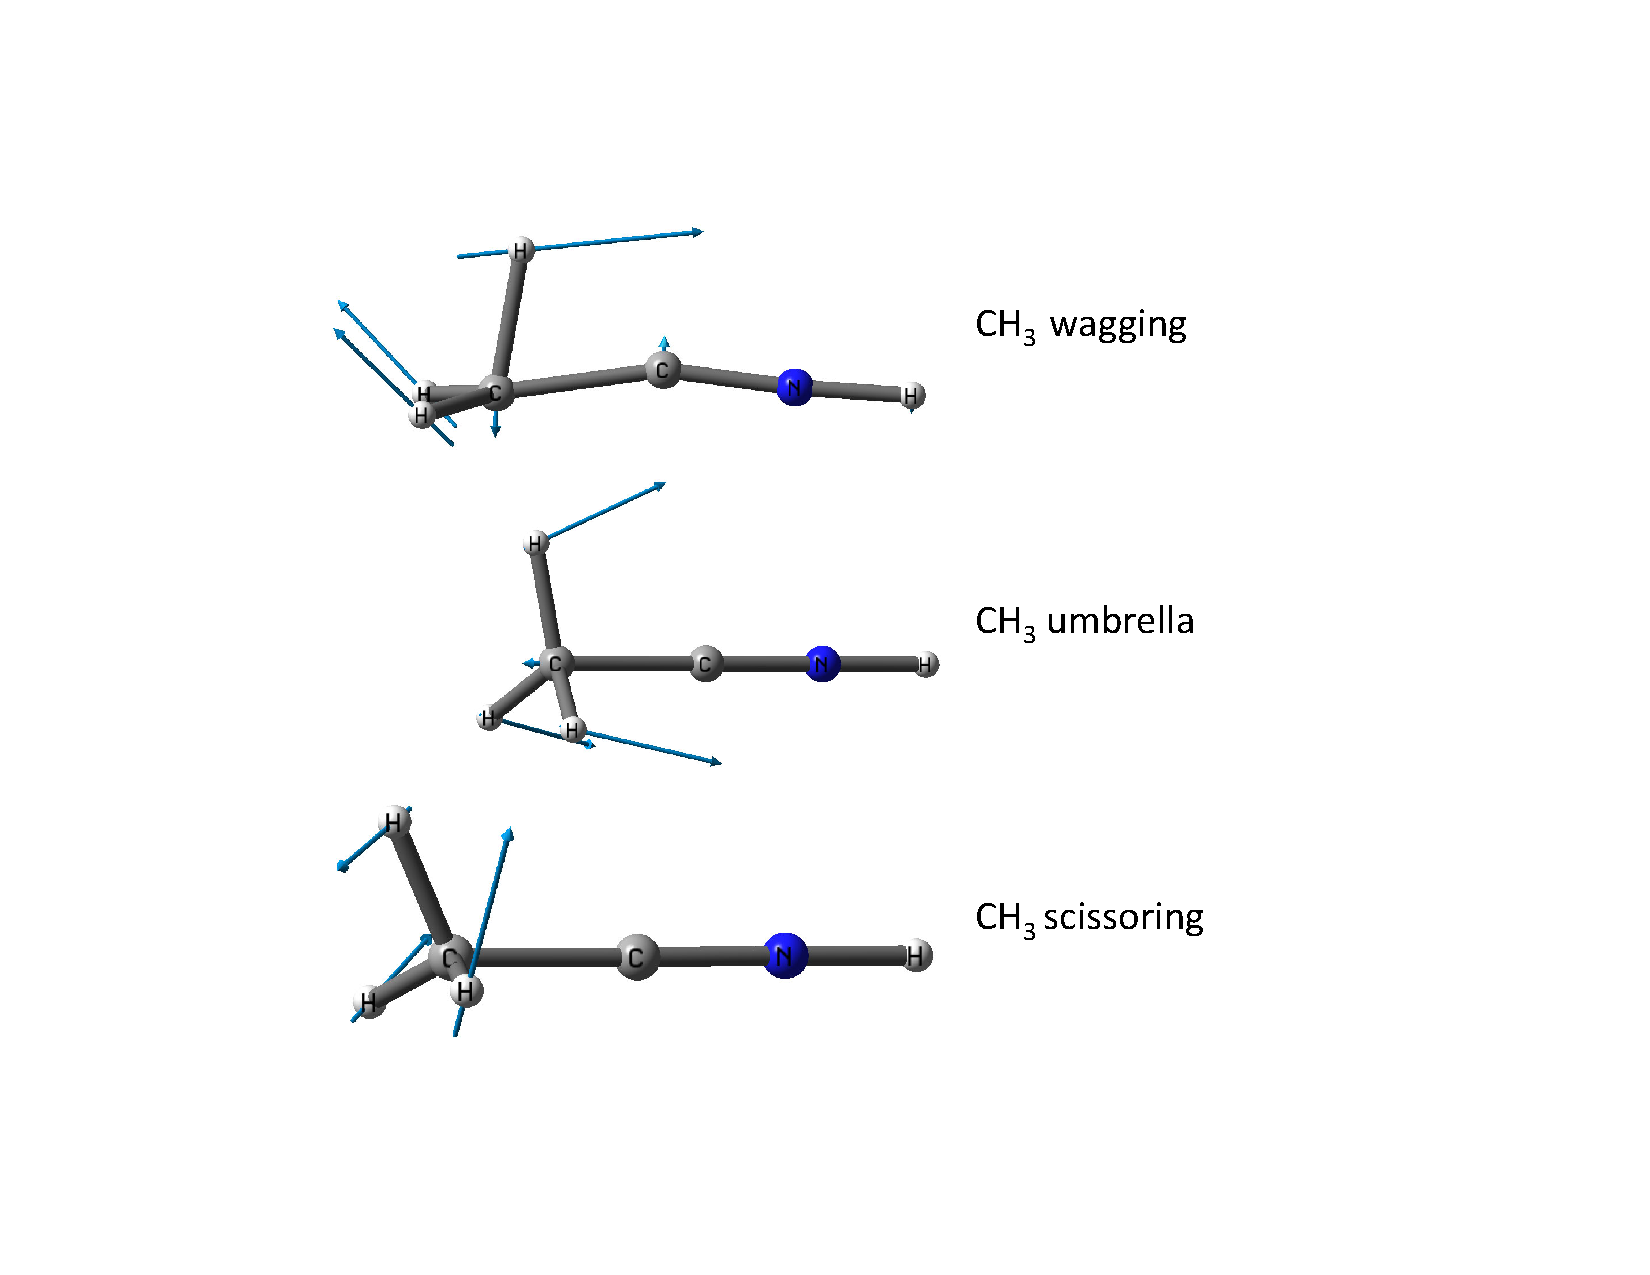
\includegraphics[scale=.5]{chapters/CH3CNH+/figures/vibration_vector.pdf}
		\caption{Vibrational displacement vectors for CH$_3$ modes.}\label{fig:CH3CNH+:fig2}
	\label{FIG:ch3_modes}
\end{figure}

\newpage
% \section{Calculated rotational spectroscopic parameters\\ at the CCSD(T)/ANO2 level of theory}

\begin{center}
    \begin{table}[h]
    \caption{Calculated spectroscopic parameters of \pa at the CCSD(T)/ANO2 level of theory. Rotational constants $B_e$, $B_0$, $\Delta B_0=1/2\Sigma \alpha^B_i$ ($\Delta A_0$ analogous), and $\alpha^A_i$ and $\alpha^B_i$. All values are in MHz.}\label{tab:CH3CNH+:tab4}
        \centering
        \begin{tabular}{cccccc}
            \hline\hline\\
            $A_e$    & $A_0$    &  $\Delta A_0$ & $B_e$  & $B_0$  & $\Delta B_0$  \\\hline\\
            156213.5 & 154336.7 & 1876.8        & 8659.2 & 8541.5 & 27.8            \\\\
            \hline\hline\\
            \multicolumn{2}{c}{mode}          & $\alpha^A_i$ & $\alpha ^B_i$ & $q_i$ & \\\hline\\
            $\nu_{10}$ & CCN bend             & 91.3  &  -20.2 & 14.8    &  \\
            $\nu_9$    & CNH bend             & 31.1  &  -8.3  & 8.9     &  \\
            $\nu_5$    & CC stretch           & 251   &  50.6  &         &  \\
            $\nu_8$    & CH$_3$ wagging       & -883  &  -0.09 & 3.6     &  \\
            $\nu_4$    & CH$_3$ umbrella      & -912  &  68.0  &         &  \\
            $\nu_7$    & CH$_3$ scissoring    & 902   &  -37.7 & 60.2    &  \\
            $\nu_3$    & CN stretch & 103     & 44.0  &        &            \\
            $\nu_2$    & CH$_3$ sym. stretch  & 1645  & 2.2    &         &  \\
            $\nu_6$    & CH$_3$ asym. stretch & 1204  & 0.99   & 0.634   &  \\
            $\nu_1$    & NH stretch           & -23.4 & 21.5   &         &  \\
            
            \hline\hline
        \end{tabular}
        \label{rot}
    \end{table}
\end{center}
% \end{subappendices}
